\documentclass{article}
\usepackage{geometry}
\usepackage{graphicx}

\geometry{a4paper, margin=1.2in} 

\begin{document}
\title{Predicting Energy of $H_2O$ Molecule\\ \large Machine Learning Assignment}

\author{Srivathsan S}
\maketitle

\section{Introduction}
\begin{flushleft}
    The Ground State Energy of a molecule is based on several factors including the number of atoms in the molecule, the type of bond between the atoms
    and the size of the atoms. This paper aims to predict the total energy of the molecule using the co ordinates of the atoms in the molecule in 3D Space
    using machine learning, particularly neural networks. We use data obtained from analytical solving of the $H_2O$ molecule energy to train the neural
    network. The importance of data pre-processing data and size of training set is also explored.
\end{flushleft}


\section{Data Pipeline}
\begin{flushleft}
    The Input Data is of the form .xyz file containing the co-ordinate geometry of the atoms in the molecule ( 1750 molecules ) and it's corresponding energy
    in a separate .ener file. The available data is of 2 types, rotated and unrotated orientations of the molecules. We first clean the data and normalize it
    using the formula :

    $$ x' = \frac{x - \bar{x}}{max(x) - min(x)} \forall x \in X \cup Y $$

    For the second approach, the convert the input data of co-ordinate points to distance between the individual atoms of the molecule by using the
    Eucledian distance formula :
    $$ d = \sqrt{(x_1 - x_2)^2 + (y_1 - y_2)^2 + (z_1 - z_2)^2} $$

    We find the distances between the 2 O-H pairs and H-H atoms prior to normalizing. Two neural networks of the same architecture are trained on these
    datasets.
\end{flushleft}


\section{Neural Network Model}
\begin{flushleft}
    We used a simple Feedforward Neural Network of the following size:

    \begin{center}
        \begin{tabular}{ |c|c|c| }
            \hline
            Layer Type & Shape & Parameters \\
            \hline
            $Input^*$  & 9     & 9          \\
            Dense      & 32    & 128        \\
            Dense      & 16    & 528        \\
            Dense      & 8     & 136        \\
            Output     & 1     & 8          \\
            \hline
        \end{tabular}
    \end{center}

    We used a sigmoid activation function on all nodes and a Stochastic Gradient Descent Algorithm with Adam Optimizer was used to learn the weights of
    the neural network. We used to learning rate of 0.001 and L2 regularization with a penalty of $1e^{-6}$ to the weights of the GDA to train faster.
    For the neural network training on the distances, only the Input Layer changes to Shape 3.
\end{flushleft}

\section{Model Performance}
\begin{flushleft}
    The model was trained for 300 epochs and the results are below: \newline
\end{flushleft}

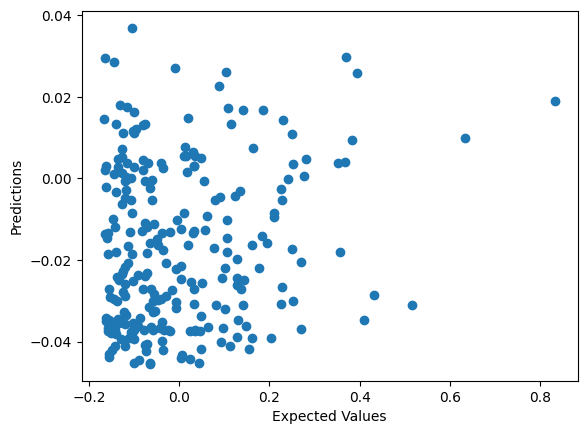
\includegraphics[scale=0.5]{../images/cord_rot.png}
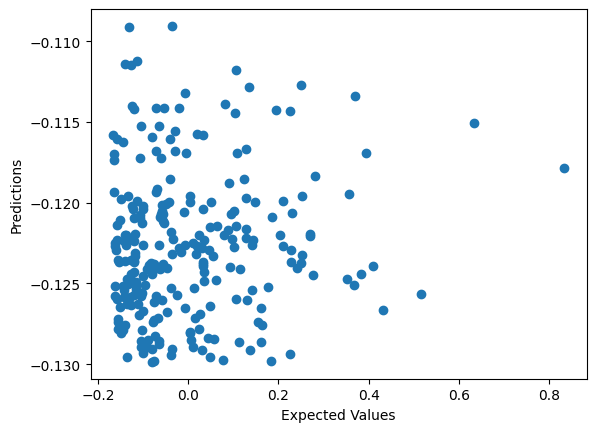
\includegraphics[scale=0.5]{../images/cord_unrot.png}
\begin{center} (a) Model Trained on Co Ordinates Data with and without Rotated Molecules Data \end{center}

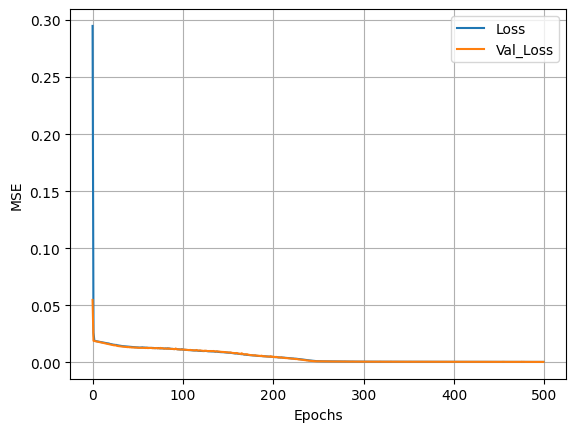
\includegraphics[scale=0.5]{../images/dist_unrot.png}
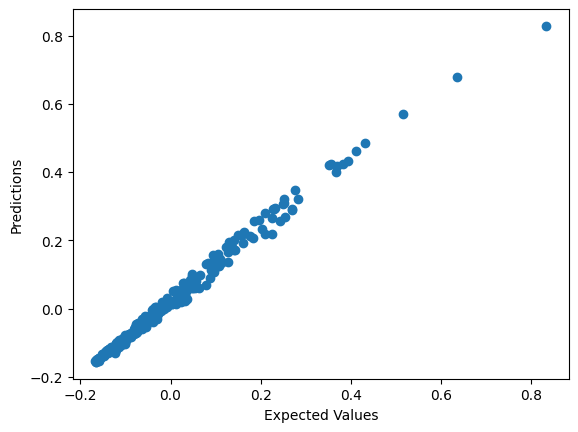
\includegraphics[scale=0.5]{../images/dist_unrot2.png}
\begin{center} (b) Model Trained on Unrotated Molecules Data with Distances \end{center}

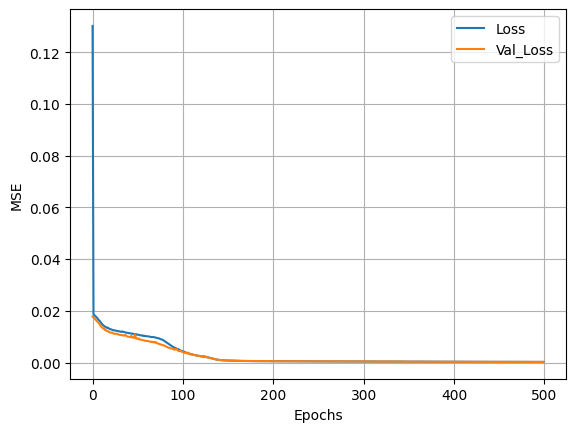
\includegraphics[scale=0.5]{../images/dist_rot.png}
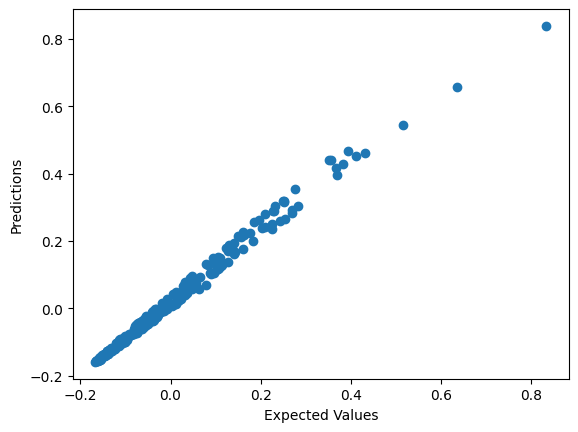
\includegraphics[scale=0.5]{../images/dist_rot2.png}
\begin{center} (c) Model Trained on Rotated + Unrotated Data with Distances \end{center}

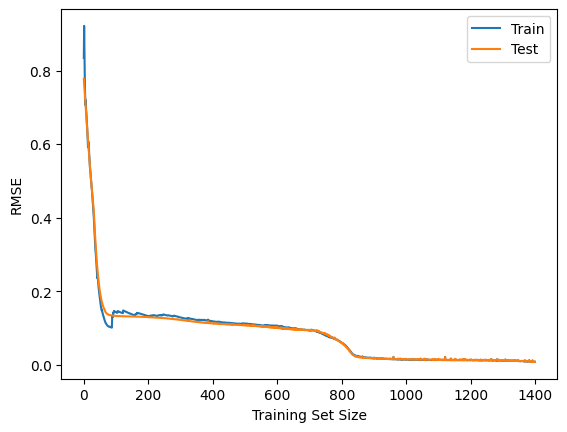
\includegraphics[scale=0.5]{../images/learning_curve.png}
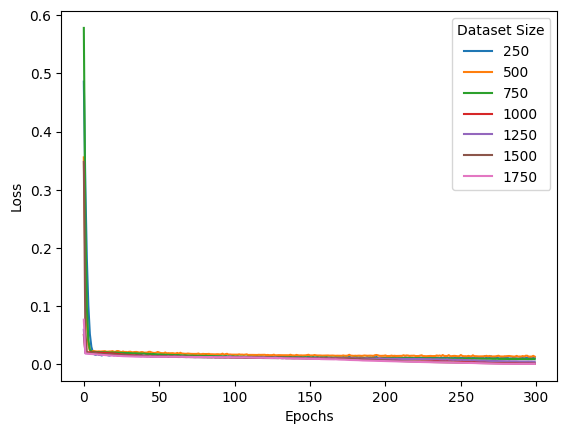
\includegraphics[scale=0.5]{../images/loss_curves.png}
\begin{center} (d) Learning Curve for Model trained in (c); and (e) Loss Curves for Models trained for Different Dataset sizes.\end{center}

\section{Inferences}
\begin{flushleft}
    \begin{enumerate}
        \item We can see that the data trained on co-ordinates data performs badly in this dataset. Even when including twice the data with the rotated dataset ( 1750*2 ), the model only perfomrs slightly better as evident from the lower spread of the data.
        \item Model trained on distances with the unrotated molecules performs exponentially better than unpreprocessed data, with a RMSE value of 0.051. The predicted pretty much lies mostly on the line $y=x$, showing near perfect prediction.
        \item Further, Model trained on both rotated and unrotated data performs better than the model trained in Fig (b) with a RMSE of 0.027. Both training and validation loss are lower than the previous model, and the predicted data has a tighter grouping than before. This is the most optimized model trained from this data.
        \item Figure (d) shows the RMSE during the training of the most optimised model (c). Both the training and test loss decreases exponentially and drops to order of $1e^{-4}$.
        \item The Loss Curves for model trained with different dataset sizes. We can see that the model trained with lesser data ( light green ) has the greatest loss. The data also starts to overfit with more epochs as evident from the increasing loss at Epochs greater than 250.
        \item The difference in the model performances of the co ordinate and distances data shows the importance of pre processing of the data. Either we have to choose the important features of the data manually or we have to use automated methods like PCA.
    \end{enumerate}
\end{flushleft}

\section{Inferences}
\begin{flushleft}
    The Given data of $H_2O$ Molecule co ordinates with their corresponding energies were analysed and used to train a neural network model. It was found that using the distance between the molecules as the input and training over a larger dataset creates the better performing model. Further, Increased accuracy can be obtaiend by deepening the model with an additional hidden layer of 64 nodes or by training over a larger dataset ( greater than 5000 datapoints ). We can also try to input additional features to train over like temperature, overall charge of the molecule etc. The good performance of the model also shows the correlation between bond distances and energy of the molecule.
\end{flushleft}
\end{document}